\chapter{Lec 15 - 16 - Shrinkage Methods}

\section{Shrinkage Methods}
The subset selection methods described in the previous chapters involve using least squares to fit a linear model that contains a subset of the predictors. As an alternative, we can fit a model containing all $p$ predictors using a technique that constrains or regularizes the coefficient estimates, or equivalently, that shrinks the coefficient estimates towards zero. It turns out that shrinking the coefficient estimates can significantly reduce their variance. The two best-known techniques for shrinking the regression coefficients towards zero are ridge regression and the lasso.

\subsection{Ridge Regression}
Ridge regression is very similar to least squares, except that the coefficients are estimated by minimizing a slightly different quantity. The ridge regression coefficient estimates $\hat{\beta}^R$ are the values that minimize
\begin{equation}
    RSS + \lambda \sum_{j=1}^p \beta_j^2
    \label{ridge-regression}
\end{equation}
where $\lambda \geq 0$ is a tuning parameter, to be determined separately. Equation \ref{ridge-regression} trades off two different criteria. As with least squares, ridge regression seeks coefficient estimates that fit the data well, by making the RSS small. However, the second term, called a shrinkage penalty, is small when $\beta_1,...,\beta_p$ are close to zero, and so it has the effect of shrinking the estimates of $\beta_j$ towards zero. The tuning parameter $\lambda$ serves to control the relative impact of these two terms on the regression coefficient estimates. When $\lambda = 0$, the penalty term has no effect, and ridge regression will produce the least squares estimates. However, as $\lambda \rightarrow \infty$, the impact of the shrinkage penalty grows, and the ridge regression coefficient estimates will approach zero. The shrinkage penalty is applied to $\beta_1,...,\beta_p$, but not to the intercept $\beta_0$. We want to shrink the estimated association of each variable with the response; however, we do not want to shrink the intercept, which is simply a measure of the mean value of the response when $x_{i1} = x_{i2} = ... = x_{ip} = 0$.

\subsubsection{An Application to the Credit Data}
In the Figure below the ridge regression coefficient estimates for the Credit data set are displayed. In the left-hand panel, each curve corresponds to the ridge regression coefficient estimate for one of the ten variables, plotted as a function of $\lambda$.
\begin{center}
    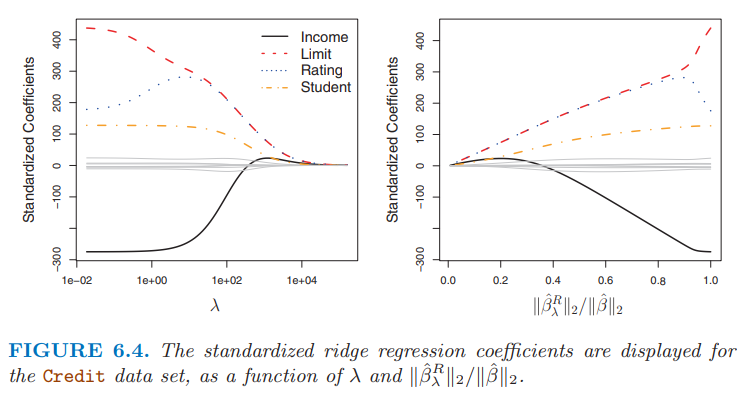
\includegraphics[scale=0.7]{images/ridge-reg.png}
\end{center}
At the extreme left-hand side of the plot, $\lambda$ is essentially zero, and so the corresponding ridge coefficient estimates are the same as the usual least squares estimates. But as $\lambda$ increases, the ridge coefficient estimates shrink towards zero. The right-hand panel of the Figure  displays the same ridge coefficient estimates as the left-hand panel, but instead of displaying $\lambda$ on the x-axis, we now display $||\hat{\beta}_\lambda^R||_2 / ||\hat{\beta}||_2$, where $\hat{\beta}$ denotes the vector of least squares coefficient estimates. The notation $||\hat{\beta}||_2$ denotes the $l_2$ norm of a vector, and is defined as $||\beta||_2 = \sqrt{\sum_{j=1}^p \beta_j^2}$. It measures the distance of $\beta$ from zero. As $\lambda$ increases, the $l_2$ norm of $\hat{\beta}_\lambda^R$ will always decreases, and so will $||\hat{\beta}_\lambda^R||_2 / ||\hat{\beta}||_2$.  The latter quantity ranges from 1 (when $\lambda = 0$) to 0 ((when $\lambda = \infty$). Therefore, we can think of the x-axis in the right-hand panel of the Figure as the amount that the ridge regression coefficient estimates have been shrunken towards zero.\\\\
The standard least squares coefficient estimates are scale invariant: multiplying $X_j$ by a constant $c$ simply leads to a scaling of the least squares coefficient estimates by a factor of $1/c$. In contrast, the ridge regression coefficient estimates can change substantially when multiplying a given predictor by a constant. Therefore, it is best to apply ridge regression after \textit{standardizing the predictors} so that they are all on the same scale.

\subsubsection{Why Does Ridge Regression Improve Over Least Squares?}
Ridge regression’s advantage over least squares is rooted in the bias-variance trade-off. As $\lambda$ increases, the flexibility of the ridge regression fit decreases, leading to decreased variance but increased bias. The green curve in the left-hand panel of the Figure below displays the variance of the ridge regression predictions as a function of $\lambda$.
\begin{center}
    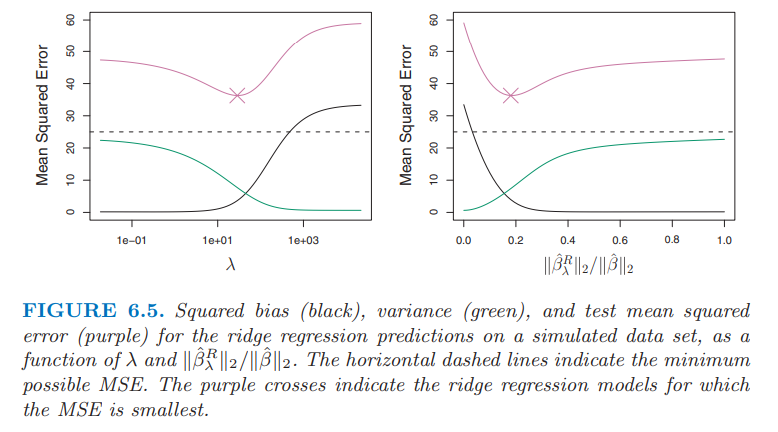
\includegraphics[scale=0.6]{images/ridge-reg-bias-variance.png}
\end{center}
At the least squares coefficient estimates, which correspond
to ridge regression with $\lambda = 0$, the variance is high but there is no bias. But as $\lambda$ increases, the shrinkage of the ridge coefficient estimates leads to a substantial reduction in the variance of the predictions, at the expense of a slight increase in bias. the MSE drops considerably as $\lambda$ increases from 0 to 10. Beyond this point, the decrease in variance due to increasing $\lambda$ slows, and the shrinkage on the coefficients causes them to be significantly underestimated, resulting in a large increase in the bias. The minimum MSE is achieved at approximately $\lambda = 30$.\\\\
Ridge regression works best in situations where the least squares estimates have high variance. Ridge regression also has substantial computational advantages over best subset selection, which requires searching through $2^p$ models. As we discussed previously, even for moderate values of $p$, such a search can be computationally infeasible. In contrast, for any fixed value of $\lambda$, ridge regression only fits a single model, and the model-fitting procedure can be performed quite quickly.

\subsection{The Lasso}
Ridge regression does have one obvious disadvantage. Unlike best subset, forward stepwise, and backward stepwise selection, which will generally select models that involve just a subset of the variables, ridge regression will include all $p$ predictors in the final model. The penalty term will shrink all of the coefficients towards zero, but it will not set any of them exactly to zero (unless $\lambda = \infty$). This may not be a problem for prediction accuracy, but it can create a challenge in model interpretation in settings in which the number of variables $p$ is quite large.\\\\
The lasso is a relatively recent alternative to ridge regression that overcomes this disadvantage. The lasso coefficients, $\hat{\beta}^L_\lambda$ , minimize the quantity
\begin{equation}
    RSS + \lambda \sum_{j=1}^p |\beta_j|
    \label{lasso}
\end{equation}
Comparing \ref{ridge-regression} to \ref{lasso}, we see that the lasso and ridge regression have similar formulations. The only difference is that the $\beta_j^2$ term in the ridge regression penalty has been replaced by $|\beta_j|$ in the lasso penalty. The lasso uses an $l_1$ penalty instead of a $l_2$ penalty. As with ridge regression, the lasso shrinks the coefficient estimates towards zero. However, in the case of the lasso, the $l_1$ penalty has the effect of forcing some of the coefficient estimates to be exactly equal to zero when the tuning parameter $\lambda$ is sufficiently large. Hence, much like best subset selection, the lasso performs \textit{variable selection}. As a result, models generated from the lasso are generally much easier to interpret than those produced by ridge regression. We say that the lasso yields \textit{sparse} models—that is, models that involve only a subset of the variables. 

\subsubsection{The Variable Selection Property of the Lasso}
Why is it that the lasso, unlike ridge regression, results in coefficient estimates that are exactly equal to zero? The figure below illustrates the situation. The least squares solution is marked as $\hat{\beta}$, while the blue diamond and circle represent the lasso and ridge regression constraints, respectively.
\begin{center}
    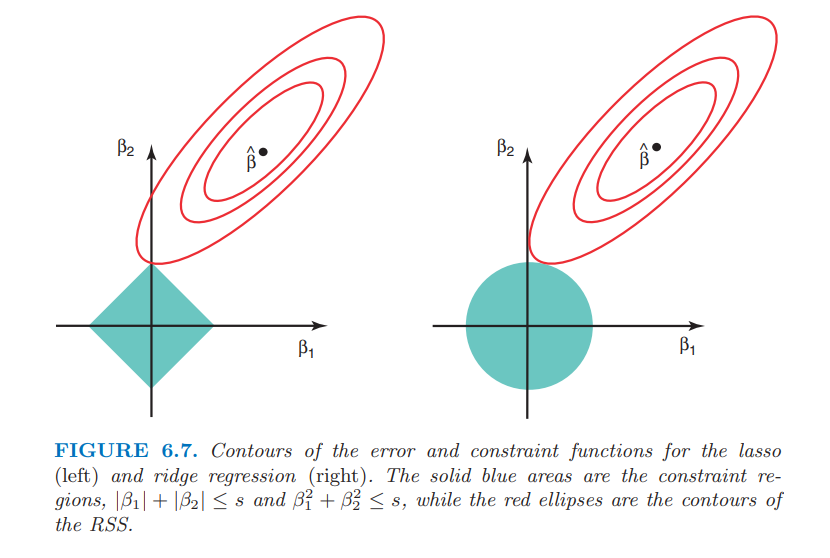
\includegraphics[scale=0.7]{images/ridge-lasso-geom.png}
\end{center}
The ellipses that are centered around $\hat{\beta}$ represent regions of constant
RSS. In other words, all of the points on a given ellipse share a common value of the RSS. As the ellipses expand away from the least squares coefficient estimates, the RSS increases. The lasso and ridge regression coefficient estimates are given by the first point at which an ellipse contacts the constraint region. Since ridge
regression has a circular constraint with no sharp points, this intersection will not generally occur on an axis, and so the ridge regression coefficient estimates will be exclusively non-zero. However, the lasso constraint has corners at each of the axes, and so the ellipse will often intersect the constraint region at an axis. When this occurs, one of the coefficients will equal zero. In higher dimensions, many of the coefficient estimates may equal zero simultaneously.

\subsection{Comparing the Lasso and Ridge Regression}
It is clear that the lasso has a major advantage over ridge regression, in that it produces simpler and more interpretable models that involve only a subset of the predictors. However, which method leads to better prediction accuracy? In general, one might expect the lasso to perform better in a setting where a relatively small number of predictors have substantial coefficients, and the remaining predictors have coefficients that are very small or that equal zero. Ridge regression will perform better when the response is a function of many predictors, all with coefficients of roughly equal size. A technique such as cross-validation can be used in order to determine which approach is better on a particular data set.

\subsection{Bayesian Interpretation for Ridge Regression and the Lasso}
We now show that one can view ridge regression and the lasso through
a Bayesian lens. A Bayesian viewpoint for regression assumes that the coefficient vector $\beta$ has some \textit{prior distribution}, say $p(\beta)$, where $\beta = (\beta_0, \beta_1,...,\beta_p)^T$. The likelihood of the data can be written as $f(Y |X, \beta)$, where $X = (X_1,...,X_p)$. Multiplying the prior distribution by the likelihood gives us (up to a proportionality constant) the \textit{posterior distribution}
\begin{equation}
    p(\beta| X, Y) \propto f(Y|X, \beta) p(\beta|X) = f(Y|X, \beta) p(\beta)
\end{equation}
where the proportionality above follows from Bayes’ theorem, and the equality above follows from the assumption that $X$ is fixed. We assume the usual linear model, and suppose that the errors are independent and drawn from a normal distribution. Furthermore, assume that $p(\beta) = \prod_{j=1}^p g(\beta_j)$, for some density
function $g$. It turns out that ridge regression and the lasso follow naturally
from two special cases of $g$:
\begin{itemize}
    \item  $g$ is a Gaussian distribution with mean zero and standard deviation a function of $\lambda$, then it follows that the posterior mode for $\beta$, that is, the most likely value for $\beta$, given the data, is given by the ridge regression solution.

    \item If $g$ is a double-exponential (Laplace) distribution with mean zero and scale parameter a function of $\lambda$, then it follows that the posterior mode for $\beta$ is the lasso solution.
\end{itemize}
Therefore, from a Bayesian viewpoint, ridge regression and the lasso follow directly from assuming the usual linear model with normal errors, together with a simple prior distribution for $\beta$.
\begin{center}
    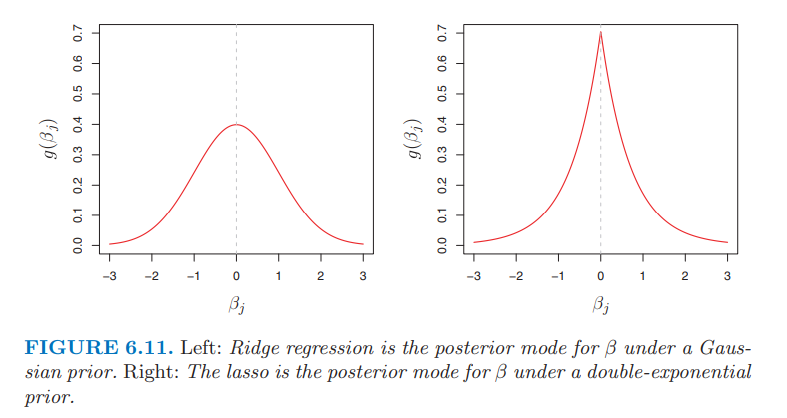
\includegraphics[scale=0.7]{images/ridge-lasso-bayesian.png}
\end{center}

Notice that the lasso prior is steeply peaked at zero, while the Gaussian is flatter and fatter at zero. Hence, the lasso expects a priori that many of the coefficients are (exactly) zero, while ridge assumes the coefficients are randomly distributed about zero.

\subsection{Selecting the Tuning Parameter}
Just as the subset selection approaches require a method to determine which of the models under consideration is best, implementing ridge regression and the lasso requires a method for selecting a value for the tuning parameter $\lambda$. Cross-validation provides a simple way to tackle this problem. We choose a grid of $\lambda$ values, and compute the cross-validation error for each value of $\lambda$. We then select the tuning parameter value for which the cross-validation error is smallest. Finally, the model is re-fit using all of the available observations and the selected value of the tuning parameter.

\section{High-Dimensional Data}
Most traditional statistical techniques for regression and classification are intended for the low-dimensional setting in which $n$, the number of observations, is much greater than $p$, the number of features. In the past 20 years, new technologies have changed the way that data are collected. While $p$ can be extremely large, the number of observations $n$ is often limited due to cost, sample availability, or other considerations.\\\\
Data sets containing more features than observations are often referred
to as \textit{high-dimensional}. Classical approaches such as least squares linear regression are not appropriate in this setting.

\subsection{What Goes Wrong in High Dimensions?}
When the number of features $p$ is as large as, or larger than, the number of observations $n$, least squares cannot (or rather,
should not) be performed. The reason is simple: regardless of whether or not there truly is a relationship between the features and the response, least squares will yield a set of coefficient estimates that result in a perfect fit to the data, such that the residuals are zero.\\\\
An example is shown in the Figure below with $p = 1$ feature (plus an intercept) in two cases: when there are 20 observations, and when there are only two observations.
\begin{center}
    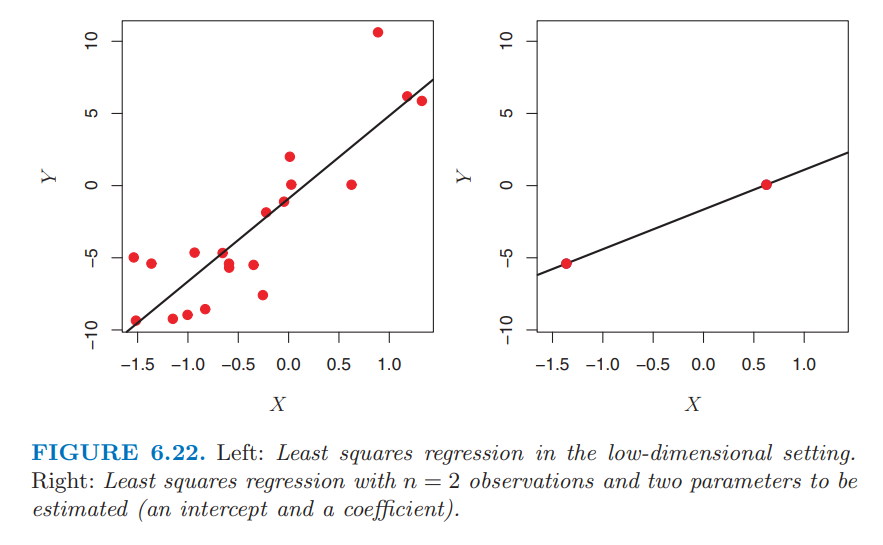
\includegraphics[scale=0.7]{images/high-dimensional.png}
\end{center}
When there are 20 observations, $n>p$, the least squares regression line does not perfectly fit the data. On the other hand, when there are only two observations, then regardless of the values of those observations, the regression line will fit the data exactly. This is problematic because this perfect fit will almost certainly lead to overfitting of the data. The problem is simple: when $p>n$ or $p \approx n$, a simple least squares regression line is too flexible and hence overfits the data.

\subsection{Regression in High Dimensions}
It turns out that many of the methods seen in this chapter for fitting
less flexible least squares models, such as forward stepwise selection, ridge regression, the lasso, and principal components regression, are particularly useful for performing regression in the high-dimensional setting. Essentially, these approaches avoid overfitting by using a less flexible fitting approach than least squares.\\\\
A key principle in the analysis of highdimensional data is the so called \textit{curse of dimensionality}. One might think that as the number of features used to fit a model increases, the quality of the fitted model will increase as well. However, this is not necessary the case. In general, adding additional signal features that are truly associated with the response will improve the fitted model, in the sense of leading to a reduction in test set error. However, adding
noise features that are not truly associated with the response will lead to a deterioration in the fitted model, and consequently an increased test set error. 
